\documentclass[journal]{IEEEtran}

\usepackage[utf8]{inputenc}
\usepackage[T1]{fontenc}
\usepackage[spanish,es-tabla,es-noquoting]{babel}
\usepackage{graphicx}
\usepackage{booktabs}
\usepackage{multirow}
\usepackage{array}
\usepackage{amsmath}
\usepackage{url}
\usepackage{xcolor}

\title{Autogeneración solar fotovoltaica en hogares de Popayán:\\
propuesta integrada de energía circular inteligente e IA (2026--2030)}

\author{Juan Pablo López\IEEEauthorblockA{Diplomado en Energía Circular Inteligente 5.0\\
Facultad de Ingeniería -- Unicomfacauca\\
Popayán, Cauca, Colombia}\\
\and Jean Sules\IEEEauthorblockA{Diplomado en Energía Circular Inteligente 5.0\\
Facultad de Ingeniería -- Unicomfacauca\\
Popayán, Cauca, Colombia}\\
\and Santiago Amú\IEEEauthorblockA{Diplomado en Energía Circular Inteligente 5.0\\
Facultad de Ingeniería -- Unicomfacauca\\
Popayán, Cauca, Colombia}}

\begin{document}
\maketitle

\begin{abstract}
La transición energética justa en Colombia requiere soluciones territorializadas que integren fuentes no convencionales de energía renovable (FNCER), eficiencia, economía circular e inteligencia artificial (IA). Este artículo formula el problema orientador del proyecto integrador del Diplomado en Energía Circular Inteligente 5.0, cuyo caso de estudio es la autogeneración fotovoltaica residencial en Popayán, Cauca. A partir de un mapa territorial argumentado, una matriz normativa de catorce disposiciones y un conjunto de datos sintético de 1.000 hogares, se diagnostican las barreras normativas, económicas, técnicas, sociales y digitales que limitan la adopción. Se integran además los resultados computacionales disponibles en el repositorio: un pipeline de analítica y aprendizaje automático, una red neuronal multimodal, un tablero web y la libreta ejecutable que genera y modela los datos. Los resultados muestran que, con datos sintéticos, el mejor clasificador alcanza AUC macro de 0,496 y F1-macro de 0,340 en prueba, y que el retorno simple depende fuertemente del estrato (11,9, 8,2 y 6,7 años). Se concluye que la articulación de comunidades energéticas, IA y economía circular constituye una vía viable para cerrar brechas energéticas, siempre que las cifras se validen con datos reales y se respete la Ley 1581 de 2012.
\end{abstract}

\begin{IEEEkeywords}
transición energética, autogeneración fotovoltaica, energía circular, inteligencia artificial, comunidades energéticas, Popayán, análisis de datos sintéticos
\end{IEEEkeywords}

\section{Introducción}
La transición energética es un eje estructurante de la política pública contemporánea. El Acuerdo de París y los Objetivos de Desarrollo Sostenible ---en particular los ODS 7, 9, 11, 12 y 13--- han impulsado la diversificación de las matrices energéticas, la reducción de gases de efecto invernadero (GEI) y el acceso universal a la energía. En Colombia, la Ley 697 de 2001 declaró el Uso Racional y Eficiente de la Energía (URE) como asunto de interés social; la Ley 1715 de 2014 reguló la integración de las FNCER al Sistema Energético Nacional; la Ley 2099 de 2021 modernizó ese marco; la Ley 2294 de 2023 incorporó la transición energética justa; y los documentos CONPES 4075 de 2022 y CONPES 4144 de 2025 articularon la transición con la política de IA \cite{r1,r2,r3,r4,r6,r7}.

Popayán, capital del Cauca, reúne condiciones favorables: radiación solar promedio de 4,48 kWh/m$^2$/día, brillo solar de 4 a 5 horas diarias y altitud de 1.800 m s.n.m. \cite{r14}. No obstante, persisten brechas: el 19,2\,\% de la población de la subcuenca del Río Molino presenta Necesidades Básicas Insatisfechas (NBI), la mayoría de los hogares se concentra en estratos 1 y 2, y la autogeneración residencial es marginal, a pesar de la existencia de parques solares a gran escala \cite{r13,r15}.

Este artículo se estructura en diez secciones. Tras la introducción se presentan el mapa territorial y el marco normativo; se formula luego el problema orientador, los objetivos y los marcos referenciales. La sección de resultados incorpora la evidencia cuantítica generada en el repositorio y la sección final resume conclusiones y recomendaciones de política.

\section{Mapa territorial argumentado}
\IEEEPARstart{E}{l} mapa territorial no es una descripción geográfica, sino una construcción analítica que articula dimensiones física, socioeconómica, ambiental, cultural, institucional y energética.

\subsection{Delimitación y caracterización}
Popayán se ubica en el suroccidente de Colombia, cordillera Central, a 2°25' de latitud norte y 76°62' de longitud oeste, con aproximadamente 512 km$^2$. Se divide en nueve comunas urbanas y veintidós corregimientos rurales. La población aproximada es de 320.000 habitantes, con un Índice de Condiciones de Vida del 82,61\,\% y coberturas de energía eléctrica, agua potable y gas natural del 98\,\%, 96,1\,\% y 63,5\,\%, respectivamente \cite{r13}. La diversidad cultural ---comunidades campesinas, pueblos Nasa y Misak, y población afrodescendiente--- exige un enfoque diferencial e interseccional, reconocido en el artículo 235 de la Ley 2294 de 2023 \cite{r4}.

\subsection{Potential solar y brechas}
La radiación solar de Popayán (4,48 kWh/m$^2$/día) supera la de ciudades europeas que han masificado la generación fotovoltaica, como Berlín (2,7) o Londres (2,5) \cite{r14}. Los meses de mayor irradiación son febrero--abril y julio--septiembre. Pese a ello, se identifican seis brechas: baja penetración de autogeneración, desconocimiento de incentivos, limitada medición bidireccional, brecha digital, pobreza energética y ausencia de cadena de gestión de residuos de aparatos eléctricos y electrónicos (RAEE).

\subsection{Actores y oportunidades}
Los actores relevantes incluyen entidades estatales (Alcaldía, Gobernación, MinEnergía, UPME, CREG, IPSE, FENOGE, FONENERGIA, SSPD), academia (Universidad del Cauca, UCC, SENA), organizaciones sociales (JAC, cabildos, consejos comunitarios) y privados (operadores, desarrolladores solares e instaladores). Entre las oportunidades sobresalen los tres parques solares inaugurados en 2024, más de 30 MW instalados por Bia Energy y Evolti, y experiencias locales de IA aplicada a la energía como SolarIQ FUP y EcoSmart Energy \cite{r16}.

\section{Marco normativo}
La matriz normativa sistematiza catorce disposiciones. La Tabla~\ref{tab:normas} resume las más relevantes; el repositorio conserva los PDF completos en el directorio \texttt{normativa/}, organizado por módulo.

\begin{table}[t]
\caption{Principales normas del marco aplicable}
\label{tab:normas}
\centering
\footnotesize
\begin{tabular}{@{}lll@{}}
\toprule
Norma & Año & Aporte principal \\
\midrule
Ley 697 & 2001 & URE e energías alternativas; crea PROURE \\
Ley 142 / 143 & 1994 & Servicios públicos domiciliarios e industria eléctrica \\
Ley 1581 & 2012 & Protección de datos personales \\
Ley 1715 & 2014 & Integración de FNCER; incentivos; FENOGE \\
Ley 1672 & 2013 & Política de gestión integral de RAEE \\
Ley 1955 & 2019 & PND 2018--2022; auditorías energéticas \\
Ley 2099 & 2021 & Moderniza Ley 1715; comunidades energéticas \\
Ley 2169 & 2021 & Carbono neutralidad y resiliencia climática \\
Ley 2294 & 2023 & PND 2022--2026; comunidades energéticas \\
Decreto 2236 & 2023 & Reglamentación de comunidades energéticas \\
Decreto 273 & 2024 & Corrección al Decreto 2236 \\
CONPES 4075 & 2022 & Política de Transición Energética \\
CONPES 4144 & 2025 & Política Nacional de Inteligencia Artificial \\
\bottomrule
\end{tabular}
\end{table}

La progresión normativa es coherente, pero existen tensiones: la Ley 2294 derogó el artículo 48 de la Ley 2099, por lo que los subsidios se rigen por el artículo 272 de la Ley 2294 hasta el 30 de junio de 2027; modificó los artículos 30 y 235 de la Ley 1715; y la reglamentación del Decreto 2236 depende aún de la CREG y del MinEnergía. Persisten vacíos en financiación accesible para estratos 1--3, trámites de certificación UPME, medición bidireccional, gestión de RAEE de paneles y baterías, y articulación regulatoria de la IA con el sector energético.

\section{Planteamiento del problema orientador}
El problema central es la \emph{baja penetración de autogeneración solar fotovoltaica en hogares de Popayán}, pese al potencial solar y al marco normativo favorable. Sus causas se agrupan en seis dimensiones: normativa (desconocimiento de incentivos y trámites complejos), económica (altos costos y falta de financiación), técnica (capacidad de instalación limitada), social (desconfianza y baja apropiación), digital (brecha de conectividad) y ambiental (ausencia de economía circular). Entre sus efectos se cuentan la pobreza energética, la dependencia de la red, la pérdida de empleo verde y el desaprovechamiento del recurso solar.

La pregunta orientadora es:
\begin{quote}
\emph{¿Cómo puede la implementación de paneles solares fotovoltaicos en hogares de Popayán, articulada con inteligencia artificial y economía circular, contribuir a la transición energética justa en el periodo 2026--2030?}
\end{quote}

Se formularon cinco subpreguntas sobre barreras, financiación mediante comunidades energéticas y fondos públicos, rol de la IA, integración de la economía circular y escalabilidad de experiencias locales. Las hipótesis H1--H4 establecen que la radiación es suficiente, que la IA y la circularidad mejoran eficiencia y sostenibilidad, que los fondos y comunidades son viables, y que la articulación de actores es condición necesaria. El problema se delimita temporalmente entre 2026 y 2030, espacialmente al municipio de Popayán y poblacionalmente a hogares de estratos 1, 2 y 3 y comunidades campesinas, indígenas y afrodescendientes.

\section{Objetivos}
El objetivo general es diseñar una propuesta de autogeneración solar fotovoltaica para hogares de Popayán, articulada con IA y economía circular, que contribuya a la transición energética justa en 2026--2030. Los objetivos específicos son: (i) caracterizar el potencial solar, socioeconómico y normativo; (ii) analizar barreras y oportunidades; (iii) evaluar el rol de la IA y la circularidad; (iv) proponer un modelo de financiación y gestión comunitaria; y (v) estimar impactos sociales, económicos y ambientales.

\section{Marco referencial y metodología}
El marco conceptual integra transición energética, FNCER, autogeneración, generación distribuida, comunidades energéticas, energía circular, IA, redes inteligentes, prosumidores y pobreza energética. La investigación es de enfoque mixto, descriptiva, explicativa, propositiva y aplicada; utiliza el estudio de caso con investigación-acción participativa, análisis normativo y análisis territorial. Las fases son caracterización, análisis normativo, diagnóstico energético y digital, diseño de la propuesta y validación. Se emplean encuestas, entrevistas, grupos focales, visitas de campo, análisis documental, análisis costo--beneficio, análisis de ciclo de vida y modelación con IA. Éticamente se exigen consentimiento informed, enfoque diferencial, protección de datos conforme a la Ley 1581 de 2012 y consulta previa cuando aplique \cite{r12}.

\section{Resultados y evidencia computacional}
Además del análisis territorial y normativo, el repositorio contiene evidencia reproducible que se integra en este artículo: un conjunto de datos de 1.000 hogares con 99 variables, una libreta de generación y modelado (\texttt{proyecto.ipynb}), un despliegue Gradio con 24 pestañas analíticas, un tablero web estático y un paquete de 108 resultados descargables.

\subsection{Datos y línea base}
El dataset sintético está calibrado con parámetros públicos de Popayán: radiación de 4,0--4,5 kWh/m$^2$/día, tarifas de 700--950 COP/kWh y estratos 1--3. La media de consumo es 111,52 kWh/mes, con distribución 650/200/150 hogares por estrato y target de disposición 40\,\% Sí, 40\,\% No y 20\,\% Tal vez. La Fig.~\ref{fig:consumo} muestra el consumo medio por estrato y la Fig.~\ref{fig:target} la disposición a instalar paneles.

\begin{figure}[t]
\centering
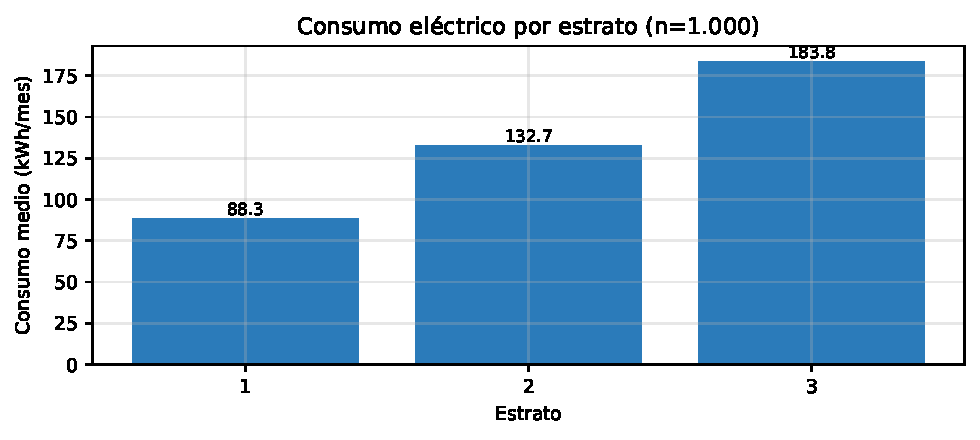
\includegraphics[width=\columnwidth]{figuras/consumo_estrato}
\caption{Consumo eléctrico medio por estrato en el dataset sintético (n=1.000).}
\label{fig:consumo}
\end{figure}

\begin{figure}[t]
\centering
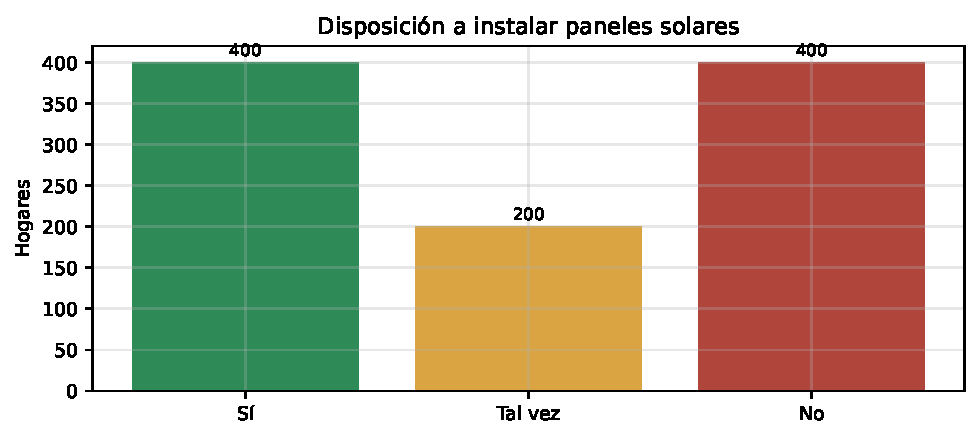
\includegraphics[width=\columnwidth]{figuras/disposicion_paneles}
\caption{Disposición declarada a instalar paneles solares.}
\label{fig:target}
\end{figure}

\subsection{Modelado y métricas}
El pipeline compara seis modelos clásicos con una red neuronal multimodal PyTorch compuesta por una rama MLP numérica, embeddings categóricos y una rama Conv1d sobre el perfil horario de 24 horas. La Tabla~\ref{tab:metricas} resume el desempeño reportado por la aplicación Gradio. El mejor clasificador por F1-macro en validación cruzada fue Regresión Logística, con AUC macro 0,496 y F1-macro 0,340 en prueba. La calibración, la importancia de variables (SHAP sobre Random Forest y Permutation Importance) y la auditoría de equidad por estrato, zona y género se encuentran en los gráficos HTML del paquete de resultados.

\begin{table}[t]
\caption{Métricas reportadas por el despliegue Gradio}
\label{tab:metricas}
\centering
\footnotesize
\begin{tabular}{@{}llr@{}}
\toprule
Indicador & Modelo & Valor \\
\midrule
AUC macro & Regresión Logística & 0,496 \\
F1-macro (prueba) & Regresión Logística & 0,340 \\
Exactitud (3 clases) & Red multimodal & 64,4\,\% \\
Exactitud (Sí/No) & Red multimodal & 77,7\,\% \\
$R^2$ ahorro anual & Cabeza de regresión & 0,98 \\
Parámetros & SolarNet-MT (web) & 9.086 \\
\bottomrule
\end{tabular}
\end{table}

\subsection{Economía y sensibilidad territorial}
El retorno simple medio difiere marcadamente entre estratos: 11,9 años en estrato 1, 8,2 en estrato 2 y 6,7 en estrato 3 (Fig.~\ref{fig:retorno}). El valor presente neto a diez años es positivo en el 0,3\,\%, 33,5\,\% y 90,7\,\% de los hogares, respectivamente. El sistema equivale a 10,6 meses de ingreso en estrato 1 frente a 2,7 en estrato 3, lo que evidencia un dilema de equidad en la asignación de subsidios: la asignación más eficiente concentra el gasto en el estrato 3, mientras que exigir equidad tiene un costo medible.

\begin{figure}[t]
\centering
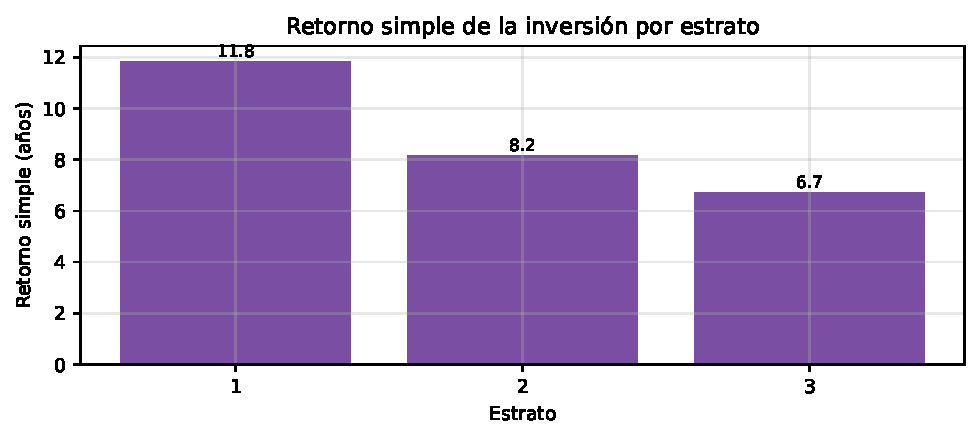
\includegraphics[width=\columnwidth]{figuras/retorno_estrato}
\caption{Retorno simple de la inversión por estrato (tablero web).}
\label{fig:retorno}
\end{figure}

\subsection{Advertencia sobre procedencia de los datos}
Los resultados descritos se obtuvieron con datos sintéticos. La libreta genera un conjunto alternativo con consumo medio de 182,6 kWh/mes y target 35/35/30, distinto del dataset versionado (111,5 kWh/mes y 40/40/20). En consecuencia, las cifras del tablero web y las de la aplicación Gradio \emph{no son directamente comparables}. Se recomienda fijar una sola fuente de datos antes de usar estos resultados en informes técnicos o sustentaciones.

\section{Impactos e indicadores de seguimiento}
Los impactos esperados son sociales (reducción de pobreza energética e inclusión), económicos (ahorro tarifario y empleo verde), ambientales (reducción de GEI y circularidad), tecnológicos (IA y recursos distribuidos) y normativos (insumos de política pública). La Tabla~\ref{tab:indicadores} presenta los indicadores de seguimiento propuestos.

\begin{table}[t]
\caption{Indicadores de seguimiento del proyecto}
\label{tab:indicadores}
\centering
\footnotesize
\begin{tabular}{@{}lrr@{}}
\toprule
Indicador & Línea base & Meta 2030 \\
\midrule
Hogares con paneles solares & 0 & 5.000 \\
Ahorro tarifario & 0\,\% & 30\,\% \\
Reducción de GEI (tCO$_2$) & 0 & 12.000 \\
Empleos verdes & 0 & 500 \\
Comunidades energéticas & 0 & 20 \\
Gestión de RAEE & 0\,\% & 80\,\% \\
Cobertura de IA & 0\,\% & 60\,\% \\
Apropiación social & 0\,\% & 70\,\% \\
\bottomrule
\end{tabular}
\end{table}

\section{Conclusiones y recomendaciones}
Popayán reúne condiciones favorables para la autogeneración solar residencial, pero persisten brechas económicas, normativas, técnicas y digitales. El marco normativo es robusto aunque presenta vacíos en financiación, trámites, medición, RAEE y regulación de IA. La articulación de comunidades energéticas, IA y economía circular constituye una vía viable para avanzar hacia un modelo de desarrollo territorial sostenible, siempre que las hipótesis se validen con datos reales anonimizados.

Se recomienda: (1) diseñar un programa municipal de autogeneración residencial articulado con FENOGE y FONENERGIA; (2) simplificar los trámites de incentivos de la Ley 1715; (3) promover comunidades energéticas; (4) integrar IA en la gestión y el monitoreo; (5) establecer una cadena de RAEE para paneles y baterías; y (6) fortalecer la capacitación y el talento digital. Como agenda futura se propone evaluar el efecto de la IA sobre la eficiencia, analizar modelos de negocio inclusivos, estudiar el RAEE de paneles solares en Colombia y medir el impacto sobre la pobreza energética.

\appendices
\section{Inventario documental del repositorio}
Toda la evidencia se conserva en el repositorio \texttt{diplomado-energia-circular-inteligente}. La Tabla~\ref{tab:artefactos} relaciona los artefactos y su ubicación.

\begin{table}[t]
\caption{Artefactos documentales disponibles}
\label{tab:artefactos}
\centering
\footnotesize
\begin{tabular}{@{}ll@{}}
\toprule
Directorio & Contenido \\
\midrule
\texttt{documento/} & Propuesta del diplomado y este artículo \\
\texttt{normativa/} & 14 PDF de leyes, decretos y CONPES \\
\texttt{datos/solar\_popayan/} & Dataset y diccionario de 99 columnas \\
\texttt{modulos/07-proyecto-integrador/notebooks/} & Libreta ejecutable \\
\texttt{modulos/07-proyecto-integrador/export\_colab/} & Exportación Python \\
\texttt{modulos/07-proyecto-integrador/sitio-web/} & Tablero desplegado en Vercel \\
\texttt{modulos/07-proyecto-integrador/gradio-app/} & Ficha y captura de la app Gradio \\
\texttt{entregables/} & ZIP con 108 resultados e inventario \\
\bottomrule
\end{tabular}
\end{table}

\section{Reproducibilidad y enlaces}
El artículo puede recompilarse con MiKTeX ejecutando \texttt{pdflatex main.tex} dos veces desde el directorio \texttt{documento/ieee/}. Las figuras se generan desde el dataset y el JSON del tablero web. Los despliegues asociados son \url{https://popayan-solar.vercel.app/} y la aplicación Gradio documentada en \texttt{modulos/07-proyecto-integrador/gradio-app/}. El token de ngrok fue redactado del código fuente y debe proporcionarse mediante la variable de entorno \texttt{NGROK\_AUTHTOKEN}.

\bibliographystyle{IEEEtran}
\begin{thebibliography}{99}
\bibitem{r1} Congreso de Colombia, ``Ley 697 de 2001,'' Diario Oficial No. 44.573, 2001.
\bibitem{r2} Congreso de Colombia, ``Ley 1715 de 2014,'' Diario Oficial No. 49.150, 2014.
\bibitem{r3} Congreso de Colombia, ``Ley 2099 de 2021,'' Diario Oficial No. 51.731, 2021.
\bibitem{r4} Congreso de Colombia, ``Ley 2294 de 2023,'' Diario Oficial No. 52.400, 2023.
\bibitem{r5} Presidencia de la República, ``Decreto 2236 de 2023,'' 2023.
\bibitem{r6} DNP, ``CONPES 4075: Política de Transición Energética,'' Bogotá, 2022.
\bibitem{r7} DNP, ``CONPES 4144: Política Nacional de Inteligencia Artificial,'' Bogotá, 2025.
\bibitem{r8} Congreso de Colombia, ``Ley 142 de 1994,'' Diario Oficial No. 41.433, 1994.
\bibitem{r9} Congreso de Colombia, ``Ley 143 de 1994,'' Diario Oficial No. 41.434, 1994.
\bibitem{r10} Congreso de Colombia, ``Ley 1955 de 2019,'' Diario Oficial No. 50.964, 2019.
\bibitem{r11} Congreso de Colombia, ``Ley 2169 de 2021,'' Diario Oficial No. 51.896, 2021.
\bibitem{r12} Congreso de Colombia, ``Ley 1581 de 2012,'' Diario Oficial No. 48.587, 2012.
\bibitem{r13} DANE, \emph{Censo Nacional de Población y Vivienda 2018}, Bogotá, 2018.
\bibitem{r14} IDEAM, \emph{Atlas de radiación solar de Colombia}, Bogotá, 2012.
\bibitem{r15} UPME, \emph{Plan Energético Nacional 2020--2050}, Bogotá, 2024.
\bibitem{r16} IPSE, ``Encuentro Transición Energética y Desarrollo Local,'' Popayán, 2024.
\bibitem{r17} Congreso de Colombia, ``Ley 1672 de 2013,'' Diario Oficial No. 48.856, 2013.
\bibitem{r18} Presidencia de la República, ``Decreto 273 de 2024,'' 2024.
\end{thebibliography}

\end{document}
